\makeatletter
\@ifundefined{ifShowAnswer}{%
  \newif\ifShowAnswer
}{}
\makeatother

% \ShowAnswerfalse
% \ShowAnswertrue

\examsetup{
  page = {
    size            = a4paper,
    show-columnline = true,
    foot-content    = {第~;~页~~共~;页\quad 数学分析II\quad 中国农业大学制}
  },
  solution = {
    show-solution = show-stay,
    % blank-type = manual,
    blank-type = none,
    % blank-vsep = 120ex plus 1ex minus 1ex
    blank-vsep = 15cm
  },
  fillin = {
    no-answer-type = none,
    show-answer = true
  },
  % style/fullwidth-stop = catcode,
  style/fullwidth-stop = false,
  % sealline = {
  %   show        = true,
  %   scope       = mod-2,
  %   circle-show = false,
  %   line-type   = solid,
  %   odd-info-content = {
  %     {\heiti \zihao{4}姓名} {\underline{\hspace*{8em}}},
  %     {\heiti \zihao{4}准考证号} {\examsquare{9}},
  %     {\heiti \zihao{4}考场号} {\examsquare{2}},
  %     {\heiti \zihao{4}座位号} {\examsquare{2}},
  %   },
  %   odd-info-xshift = 12mm,
  %   text = {此卷只装订不密封},
  %   text-width = 0.98\textheight,
  %   text-format  = \zihao{-3}\sffamily,
  %   text-xshift = 20mm
  % },
  question/show-points = true,
  paren = {
    show-answer = true
  },
  square = {
    x-length = 1.8em,
    y-length = 1.6em
  },
  font = times
}

\ifShowAnswer
\examsetup{
  solution/show-solution = show-stay,
  fillin/show-answer = true,
  paren/show-answer = true,
  page/size = a3paper
}
\else
\examsetup{
  solution/show-solution = hide,
  fillin/show-answer = false,
  paren/show-answer = false,
  page/size = a4paper,
  page/show-head = true,
  page/head-content = {
  \fancyhead[LE]{\xiaosihao 学院:\rule[-0.45mm]{2.5cm}{0.15mm} \hspace{0.0cm} 班级:\rule[-0.45mm]{2.5cm}{0.15mm} \hspace{0.0cm} 学号:\rule[-0.45mm]{3.5cm}{0.15mm} \hspace{0.0cm} 姓名:\rule[-0.45mm]{2.5cm}{0.15mm}}
  }
}
\fi


\ifShowAnswer
% do nothing
\else
\AtEndPreamble{%
\geometry{
left=20mm,
right=20mm,
top=20mm,
bottom=20mm,
% includehead=true,
% includefoot=true,
% heightrounded,
% showframe,% <--- just for debugging
% verbose,% <--- just for debugging
headsep=8pt
}
}
\fi


\title{
\erhao
\simli
\ifUseImageTitle
{
\includegraphics[height=0.85\baselineskip]{figures/logo_cau_name.png}}\\
\else
中国农业大学\\
\fi
2024\textasciitilde 2025学年春季学期\\
\textbf{%
% \uline{\hspace{1.5cm}数学分析II\hspace{1.5cm}}}
\dunderline[-1pt]{0.9pt}{\hspace{0.5cm}数学分析II\hspace{0.5cm}}}
\ifShowAnswer
课程期中考试试题解答
\else
课程期中考试试题
\fi
}

\begin{document}

\maketitle

\ifShowAnswer
% do nothing
\else
\vspace{-1.1cm}

{
\begin{table}[H]
\sihao
\centering
\begin{tabular}{|wc{2cm}|wc{2cm}|wc{2cm}|wc{2cm}|wc{2cm}|wc{2.5cm}|}
\hline
题号 & 一 & 二 & 三 & 四 & 总分 \\ \hline
分数 & & & & & \\[12pt] \hline
\end{tabular}
\end{table}
}

\vspace{-1.1cm}

\begin{center}
% \textbf{\larger 全卷满分 100 分。考试用时 100 分钟。}
{\sihao (本试卷共~4~道大题)}
\end{center}

\vspace{-1.1cm}
\begin{center}
\textbf{\sihao 考生诚信承诺}
\end{center}
\vspace{-0.5cm}
% {\sihao 本人承诺自觉遵守考试纪律,诚信应考,服从监考人员管理。\\
% 本人清楚学校考试考场规则,如有违纪行为,将按照学校违纪处分规定严肃处理。}
% 注意,这里不强行超过 linewidth 的话,第二行会自动断行
\noindent\begin{minipage}[t]{1.05\linewidth}
{\sihao 本人承诺自觉遵守考试纪律,诚信应考,服从监考人员管理。\\
本人清楚学校考试考场规则,如有违纪行为,将按照学校违纪处分规定严肃处理。}
\end{minipage}

\fi


% \begin{xiaosihao}


\section{%
  选择题:本题共 5 小题, 每小题 3 分, 共 15 分。
  在每小题给出的四个选项中, 只有一项是符合题目要求的。
}

% \noindent\scoringbox

\begin{question}
设 $f(x)$ 是定义在闭区间 $[a, b]$ 上的实值函数. 以下说法正确的是 \paren[A]

\begin{choices}
\item 若 $f(x)$ 在 $[a, b]$ 上黎曼可积, 则 $|f(x)|$ 必然也在 $[a, b]$ 上黎曼可积.
\item 若 $|f(x)|$ 在 $[a, b]$ 上黎曼可积, 则 $f(x)$ 必然也在 $[a, b]$ 上黎曼可积.
\item 若 $f(x)$ 在 $[a, b]$ 的任意子区间 $[a, c]$ 上黎曼可积, $a < c < b,$ 且极限 $\displaystyle \lim_{c\to b-} \int_a^c f(x) ~ \mathrm{d} x$ 存在, 则 $f(x)$ 必然也在 $[a, b]$ 上黎曼可积.
% \item 若 $f(x)$ 在 $[a, b]$ 上黎曼可积, 则 $f(x)$ 至多有可列多个间断点.
\item 若 $f(x)$ 在 $[a, b]$ 上黎曼可积, 改变 $f(x)$ 至多可列多个点上的取值, 则 $f(x)$ 在 $[a, b]$ 上的可积性与积分值都不变.
\end{choices}
\end{question}

\begin{solution}
B 的反例: $f(x) = 2 D(x) - 1,$ 其中 $D(x)$ 为 $[0, 1]$ 区间上的狄利克雷函数, $f(x)$ 不是黎曼可积的, 但 $|f(x)|$ 为常值函数 $1.$

C 的反例: $\displaystyle f(x) = \begin{cases} 1/\sqrt{1- x}, & 0 \leqslant x < 1, \\ 0, & x = 1. \end{cases}$

% D 的反例: 设 $P_0$ 为 $[0, 1]$ 区间上的康托三分集, $G_0$ 是其补集, $f(x) = \begin{cases} 1, & x \in P_0, \\ 0, & x \in G_0, \end{cases}$ 为 $P_0$ 的特征函数. 容易证明 $f(x)$ 的间断点集等于 $P_0,$ 是零测集, 故 $f(x)$ 黎曼可积, 但 $P_0$ 具有连续统的势. 这个选项关键点在于函数黎曼可积能推出它几乎处处连续, 即它的间断点集是零测集, 但零测集不一定要至多可列, 具有连续统势的集合也可能是零测集.
D 的反例: $[a, b] = [0, 1],$ $f(x) = 0$ 为常值函数, 将它在有理点的取值改为 $1,$ 则变为狄利克雷函数, 不可积.
\end{solution}

\begin{question}
极限 $\displaystyle \lim_{n\to\infty} \int_0^1 \left( 1 - x^{2025} \right)^n ~ \mathrm{d}x =$ \paren[D]

\begin{choices}
\item $1$
\item $\dfrac{2025}{2026}$
\item $\dfrac{1}{2026}$
\item $0$
\end{choices}
\end{question}

\begin{solution}
将积分区间拆分为 $[0, \delta]$ 与 $[\delta, 1]$ 去考虑. 或者直接利用有界收敛定理.
\end{solution}

\begin{question}
设反常积分 $\displaystyle \int_1^{+\infty} f(x) ~ \mathrm{d}x$ 收敛, 则以下论断\chemph{一定不}成立的是 \paren[B]

\begin{choices}
\item 反常积分 $\displaystyle \int_1^{+\infty} | f(x) | ~ \mathrm{d}x$ 收敛
\item 反常积分 $\displaystyle \int_1^{+\infty} \dfrac{f(x)}{x} ~ \mathrm{d}x$ 发散
\item 级数 $\displaystyle \sum_{n=1}^{\infty} f(n)$ 收敛
\item $\displaystyle \lim_{n\to\infty} \int_n^{n+1} f(x) ~ \mathrm{d}x = 0.$
\end{choices}
\end{question}

\begin{solution}
A, C 都是可能会成立, D 由柯西收敛准则必定成立, B 中的反常积分由阿贝尔-狄利克雷准备是必定收敛的.
\end{solution}

\begin{question}
以下数项级数或者无穷乘积\chemph{发散}的是 \paren[D]

\begin{choices}
\item $\displaystyle \sum_{n=1}^{\infty} ~ (-1)^n \dfrac{1}{\sqrt{n}}$
\item $\displaystyle \sum_{n=1}^{\infty} ~ \dfrac{1}{n!}$
\item $\prod_{n=1}^{\infty} ~ \dfrac{n^2}{n^2+1}$
\item $\displaystyle \prod_{n=1}^{\infty} ~ \dfrac{n}{n+1}$
\end{choices}
\end{question}

\begin{solution}
D 中的无穷乘积发散到 $0.$
\end{solution}

\begin{question}
设 $f(x)$ 是闭区间 $[a, b]$ 上的黎曼可积函数, $g(x)$ 在 $[a, b]$ 上除有限个点外可微且 $g(x) > 0$ 在 $[a, b]$ 上恒成立, $h(x)$ 是 $[a, b]$ 映射到 $[a, b]$ 自身 (不一定满射) 的连续函数. 以下函数必然黎曼可积的是 \paren[C]

\begin{choices}
\item $\dfrac{f(x)}{g(x)}$
\item $g'(x)$ (在不可微点补充定义导数值为 $0$)
\item $\max \{ f(x), g(x) \}$
\item $f \circ h(x) := f(h(x))$
\end{choices}
\end{question}

\begin{solution}
C成立的原因: $\max \{ f(x), g(x) \} = \dfrac{f(x) + g(x) + |f(x) - g(x)|}{2}.$

A 的反例: $[a, b] = [-1, 1],$ $g(x) = \begin{cases} 
x, & x \neq 0, \\ 1, & x = 0. \end{cases}$

B 的反例: $g(x) = x^2 \sin\frac{1}{x^2},$ 或者 Volterra 函数.

D 的反例构造涉及 Cantor 集: $[a, b] = [0, 1],$ $f(x) = \begin{cases} 0, & x > 0, \\ 1, & x = 0. \end{cases},$ 任取一个 $[0, 1]$ 区间内的测度大于零的类 Cantor 集 $P,$ 并取 $\displaystyle h(x) = d(x, P) = \inf_{y\in P} |x - y|,$ 那么 $h(x)$ 是连续函数, 在 $P$ 上取值恒为零, 在 $P$ 之外取值大于零. 于是 $f\circ h(x) = \begin{cases} 1, & x \in P, \\ 0, & x \not \in P, \end{cases}$ 为类 Cantor 集 $P$ 的特征函数, 间断点集为 $P.$ 由函数黎曼可积的勒贝格判别法知 $f\circ h$ 不是黎曼可积的.
\end{solution}


\section{填空题:本题共 5 小题, 每小题 3 分, 共 15 分。}

\examsetup{
  question/index = 1
}

% \noindent\scoringbox

\begin{question}
极限 $\displaystyle \lim_{n\to\infty} \left( \dfrac{n}{(n+1)^2} + \cdots + \dfrac{n}{(2n)^2} \right) =$ \fillin[$1/2$].
\end{question}

\begin{solution}
将极限表示为定积分的定义式:
\begin{equation*}
\begin{aligned}
\lim_{n\to\infty} \left( \dfrac{n}{(n+1)^2} + \cdots + \dfrac{n}{(2n)^2} \right) & = \lim_{n\to\infty} \dfrac{1}{n}\left( \dfrac{1}{(1+1/n)^2} + \cdots + \dfrac{1}{(1+n/n)^2} \right) \\
& = \int_0^1 \dfrac{1}{(1 + x)^2} ~ \mathrm{d}x = \left. -\dfrac{1}{1+x} \right|_0^1 = \dfrac{1}{2}
\end{aligned}
\end{equation*}
\end{solution}

\begin{question}
计算定积分的值 $\int_{1}^{2} \sqrt{4 - x^2} ~ \mathrm{d} x = $ \fillin[$\dfrac{2\pi}{3} - \dfrac{\sqrt{3}}{2}$]
\end{question}

\begin{solution}
这个定积分是以原点为圆心, $2$ 为半径的圆在第一象限 $0 - 60^\circ$ 扇形的面积 $\dfrac{60}{360} \cdot \pi \cdot 2^2,$ 减去相应直角三角形面积 $\dfrac{1}{2} \cdot \sqrt{3} \cdot 1.$

这题也可以利用 Newton-Leibniz 公式, 先求原函数
\begin{align*}
\int \sqrt{4 - x^2} ~ \mathrm{d} x & = x \sqrt{4 - x^2} - \int x ~ \mathrm{d} \sqrt{4 - x^2} = x \sqrt{4 - x^2} - \int x \dfrac{-2x}{2\sqrt{4 - x^2}} ~ \mathrm{d} x \\
& = x \sqrt{4 - x^2} + \int \dfrac{x^2}{\sqrt{4 - x^2}} ~ \mathrm{d} x = x \sqrt{4 - x^2} - \int \sqrt{4 - x^2} ~ \mathrm{d} x + \int  \dfrac{4}{\sqrt{4 - x^2}} ~ \mathrm{d} x,
\end{align*}
得 $\int \sqrt{4 - x^2} ~ \mathrm{d} x = \dfrac{x \sqrt{4 - x^2}}{2} + 2 \arcsin \dfrac{x}{2} + C,$ 再代入积分上下限相减.
\end{solution}

\begin{question}
若数项级数 $\displaystyle \sum_{n=1}^{\infty} (-1)^n\dfrac{1}{n^s}$ 收敛, 则实数 $s$ 的取值范围为 \fillin[$s > 0$].
\end{question}

\begin{solution}
$s > 0$ 时由 Leibniz 判别法可知收敛, $s \leqslant 0$ 时通项不趋于 $0$ 所以不收敛.
\end{solution}

\begin{question}
求数项级数的和 $\displaystyle \sum_{n=0}^{\infty} \sum_{k=0}^n \dfrac{(-1)^k}{k!(n-k)!} =$ \fillin[1].
\end{question}

\begin{solution}
题目是两个绝对收敛级数的柯西乘积:
$$\sum_{n=0}^{\infty} \sum_{k=0}^n \dfrac{(-1)^k}{k!(n-k)!} = \left( \sum_{n=0}^{\infty} \dfrac{(-1)^n}{n!} \right) \cdot \left( \sum_{n=0}^{\infty} \dfrac{1^n}{n!} \right) = e^{-1} \cdot e = 1.$$
\end{solution}

\begin{question}
已知反常积分 $\int_0^{+\infty} \dfrac{\sin x}{x} \mathrm{d} x = \dfrac{\pi}{2},$ 那么 $\int_0^{+\infty} \dfrac{\sin^3 x}{x} \mathrm{d} x =$ \fillin[$\dfrac{\pi}{4}$].
\end{question}

\begin{solution}
由三倍角公式 $\displaystyle \sin(3x) = 3\sin x - 4\sin^{3} x,$ 有
\begin{equation*}
\begin{aligned}
\int_0^{+\infty} \dfrac{\sin^3 x}{x} \mathrm{d} x & = \int_0^{+\infty} \dfrac{3\sin x - \sin(3x)}{4x} \mathrm{d} x \\
& = \dfrac{3}{4} \int_0^{+\infty} \dfrac{\sin x}{x} \mathrm{d} x - \dfrac{1}{4} \int_0^{+\infty} \dfrac{\sin (3x)}{3x} \mathrm{d} (3x) \\
& = \dfrac{3}{4} \cdot \dfrac{\pi}{2} - \dfrac{1}{4} \cdot \dfrac{\pi}{2} = \dfrac{\pi}{4}.
\end{aligned}
\end{equation*}
\end{solution}


\section{计算题:本题共 2 小题, 共 20 分。本题应写出具体演算步骤。}

\examsetup{
  question/index = 1
}

\begin{question}[points = 10]
计算定积分 $\displaystyle I = \int_0^2 \dfrac{(x-1)^2 + 1}{(x-1)^2 + x^2(x-2)^2} \mathrm{d} x.$

% \noindent\scoringbox
\end{question}

\begin{solution}
令 $t = x - 1,$ 则有
\begin{equation*}
\begin{aligned}
I & = \int_{-1}^1 \dfrac{t^2 + 1}{t^2 + (t+1)^2(t-1)^2} \mathrm{d} t \\
& = \int_{-1}^1 \dfrac{t^2 + 1}{t^2 + (t^2 - 1)^2} \mathrm{d} t = 2 \int_0^1 \dfrac{t^2 + 1}{t^2 + (t^2 - 1)^2} \mathrm{d} t \\
& = 2 \int_0^1 \dfrac{1}{(t / (1 - t^2))^2 + 1} \cdot \dfrac{1 + t^2}{(1 - t^2)^2} \mathrm{d} t \\
& = 2 \int_0^1 \dfrac{1}{(t / (1 - t^2))^2 + 1} \mathrm{d} \left( \dfrac{t}{1 - t^2} \right) \\
& = 2 \arctan \dfrac{t}{1 - t^2} \Big|_0^1 = 2 \cdot \dfrac{\pi}{2} = \pi.
\end{aligned}
\end{equation*}
\end{solution}


\begin{question}[points = 10]
由曲线 $y=\sin x$, 直线 $x=0$, $x=\frac{\pi}{2}$, 以及 $y=t (0\leqslant t \leqslant 1)$, 围成的区域面积记为 $S(t),$ 求$S(t)$的最大值与最小值.

% \noindent\scoringbox
\end{question}

\begin{solution}
先把图画出来, 可以看到灰色部分就是要求的面积, 分为了两部分:
\begin{center}
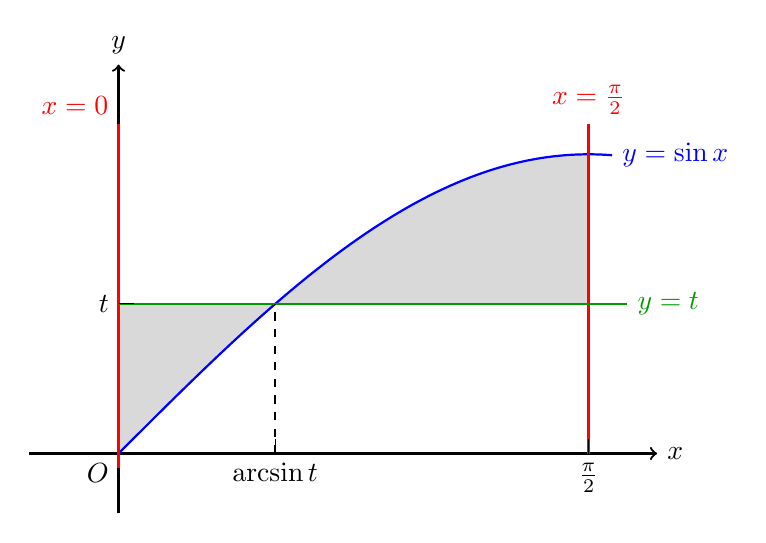
\begin{tikzpicture}[scale=3.8,declare function={f(\x)=sin(\x r);}]
 
% 坐标系
\draw[->,thick] (-0.3,0) -- (1.8,0) node[right] {$x$};
\draw[->,thick] (0,-0.2) -- (0,1.3) node[above] {$y$};
\node[below left] at (0,0) {$O$};

\def\t{0.5} % 设置 t = 0.5
\pgfmathsetmacro{\intersection}{pi/6}
 
% 填充区域(分两段闭合路径)
\fill[gray!30] 
    (0,\t) -- (\intersection,\t) 
    -- plot[domain=\intersection:0,smooth] (\x,{f(\x)}) -- cycle; % 下方区域
\fill[gray!30] 
    (\intersection,\t) -- plot[domain=\intersection:pi/2,smooth] (\x,{f(\x)}) 
    -- (pi/2,\t) -- cycle; % 上方区域
 
% 曲线与直线绘制
\draw[blue,thick] plot[domain=0:1.65,samples=50,smooth] (\x,{f(\x)}) 
    node[right] {$y=\sin x$};
\draw[red,thick] (0,-0.05) -- (0,1.1) node[above left] {$x=0$};
\draw[red,thick] (pi/2,0) -- (pi/2,1.1) node[above] {$x=\frac{\pi}{2}$};
\draw[green!60!black,thick] (0,\t) -- (1.7,\t) node[right] {$y=t$};
\draw[dashed, thick] (\intersection,0) -- (\intersection,\t);
 
% 刻度标注
\draw (pi/2,0) node[below] {$\frac{\pi}{2}$} -- (pi/2,0.05);
\draw (0,\t) node[left] {$t$} -- (0.05,\t);
\draw (\intersection,0) node[below] {$\arcsin t$} -- (\intersection,0.05); % 交点标注
 
\end{tikzpicture}
\end{center}
所以面积
\begin{align*}
S(t) & = \int_0^{\arcsin t} (t - \sin x) ~ \mathrm{d}x + \int_{\arcsin t}^{\pi/2} (\sin x - t) ~ \mathrm{d}x \\
& = (tx + \cos x)\bigg|_0^{\arcsin t} + (-\cos x - tx)\bigg|_{\arcsin t}^{\pi/2} \\
& = \bigg( t\cdot\arcsin t + \cos(\arcsin t) - 1 \bigg) + \bigg( -t \cdot \frac{\pi}{2} + \cos(\arcsin t) + t\cdot\arcsin t \bigg) \\
& = 2t\cdot\arcsin t + 2\sqrt{1 - t^2} - \frac{t\pi}{2} - 1
\end{align*}
对 $t$ 求导得 $S'(t) = 2\arcsin t - \frac{\pi}{2},$ 所以在 $t = \frac{\sqrt{2}}{2}$ 时 $S(t)$ 有最小值: $S(\frac{\sqrt{2}}{2}) = \sqrt{2} - 1.$

端点处的值 $S(0) = 1, S(1) = \frac{\pi}{2} - 1,$ 所以在 $t = 0$ 时 $S(t)$ 有最大值: $S(0) = 1.$

注意, 这题很容易从图上看出, 随着 $t$ 从 $0 \to 1$ 的过程, 右边减小的面积是递减的, 左边增加的面积是递增的, 二者达到平衡的时候正好是 $y = \sin x$ 与 $y = t$ 的交点能把线段 $y = t, 0 \leqslant x \leqslant \dfrac{\pi}{4}$ 等分的时候, 此时有 $x = \dfrac{\pi}{4}, t = y = \sin x = \dfrac{\sqrt{2}}{2}.$
\end{solution}


\section{解答题:本题共 5 小题, 共 50 分。解答应写出文字说明或者证明过程。}

\examsetup{
  question/index = 1
}

\begin{question}[points = 8]
请问 $[0, 1]$ 区间上的狄利克雷函数
\begin{equation*}
D(x) = \begin{cases} 1, & x \in \mathbb{Q} \cap [0, 1], \\ 0, & x \in [0, 1] \setminus \mathbb{Q}, \end{cases}
\end{equation*}
是否黎曼可积? 若是, 请求出积分值; 若否, 请说明原因.

% \noindent\scoringbox
\end{question}

\begin{solution}
不可积. 原因可以写以下之一:
\begin{itemize}
\item[\ding{43}] 对 $[0, 1]$ 区间的任何一个划分的任何一个小区间上, 振幅恒等于 $1;$
\item[\ding{43}] $D(x)$ 的达布上、下积分 (达布大、小和的极限) 不相等, 前者为 $1,$ 后者为 $0;$
\item[\ding{43}] $D(x)$ 在整个 $[0, 1]$ 区间上都是间断的, 间断点集 $[0, 1]$ 区间非零测集.
\end{itemize}
\end{solution}

\begin{question}[points = 10]
考虑级数 $\displaystyle \sum_{n=1}^{\infty} a_n,$ 记 $\displaystyle s_n = \sum_{k=1}^{n} a_k$ 为其前 $n$ 项和, $\displaystyle \sigma_n = \dfrac{1}{n} \sum_{k=1}^{n} s_k.$
\begin{enumerate}
\item 请证明: 若 $\displaystyle \sum_{n=1}^{\infty} a_n = A$ 收敛, 那么 $\displaystyle \lim_{n\to\infty} \sigma_n = A.$
\item 请问反过来是否成立? 即若 $\displaystyle \lim_{n\to\infty} \sigma_n = A,$ 是否能推出 $\displaystyle \sum_{n=1}^{\infty} a_n = A$? 若是, 请给出证明; 若否, 请给出反例.
\end{enumerate}

% \noindent\scoringbox
\end{question}

\begin{solution}
\begin{enumerate}
\item 由 Stolz 定理, 有
\begin{equation*}
\lim_{n\to\infty} \sigma_n = \lim_{n\to\infty} \dfrac{1}{n} \sum_{k=1}^{n} s_k = \lim_{n\to\infty} \dfrac{\sum\limits_{k=1}^{n+1} s_k - \sum\limits_{k=1}^{n} s_k}{(n+1) - n} = \lim_{n\to\infty} s_{n+1} = A.
\end{equation*}
\item 不一定. 例如 $a_n = (-1)^{n-1},$ 那么 $\displaystyle \sum_{n=1}^{\infty} a_n$ 发散, 但容易算得 $\displaystyle \lim_{n\to\infty} \sigma_n = \dfrac{1}{2}.$
\end{enumerate}
\end{solution}

\begin{question}[points = 10]
设函数 $f(x)$ 在闭区间 $[a - 1, b + 1]$ 上黎曼可积, 并且对于所有 $-1 \leqslant h \leqslant 1,$ 记 $f_h(x) = f(x + h)$ 为定义在闭区间 $[a, b]$ 上的函数. 证明:
$$\lim_{h \to 0} \int_a^b |f_h(x) - f(x)| ~ \mathrm{d} x = 0.$$

% \noindent\scoringbox
\end{question}

\begin{solution}
由振幅判别法, 对任意 $\varepsilon > 0,$ 总存在 $\delta > 0,$ 使得对 $[a-1, b+1]$ 区间上任意满足 $\lambda(P) < \delta$ 的划分 $P,$ 总有
\begin{equation*}
\sum_{i=1}^n \omega(f; [x_{i-1}, x_i]) \cdot (x_i - x_{i-1}) < \varepsilon,
\quad \omega(f; [x_{i-1}, x_i]) := \sup_{t_1, t_2 \in [x_{i-1}, x_i]} |f(t_2) - f(t_1)|.
\end{equation*}

任取 $h$ 满足 $|h| < \delta / 2,$ 并取 $[a, b]$ 的划分
\begin{equation*}
a < a + |h| < a + 2|h| < \cdots < a + k |h| < b, \quad k = \left\lceil \frac{b-a}{|h|} \right\rceil - 1.
\end{equation*}
为了记号方便, 以下不妨设 $h > 0.$ 那么在区间 $[a + (i-1)h, a + ih]$ 上恒有
\begin{equation*}
|f(x+h) - f(x)| \leqslant \omega(f; [a + (i-1)h, a + (i+1)h]),
\end{equation*}
从而有
\begin{equation*}
\begin{aligned}
\int_a^b |f(x+h) - f(x)| ~ \mathrm{d} x
& = \sum_{i=1}^k \int_{a + (i-1)h}^{a + ih} |f(x+h) - f(x)| ~ \mathrm{d} x + \int_{a + kh}^{b} |f(x+h) - f(x)| ~ \mathrm{d} x \\
& \leqslant \sum_{i=1}^{k+1} \int_{a + (i-1)h}^{a + ih} |f(x+h) - f(x)| ~ \mathrm{d} x \\
& \leqslant \sum_{i=1}^{k+1} \int_{a + (i-1)h}^{a + ih} \omega(f; [a + (i-1)h, a + (i+1)h]) ~ \mathrm{d} x \\
& = \sum_{i=1}^{k+1} \omega(f; [a + (i-1)h, a + (i+1)h]) \cdot h \\
& = \dfrac{1}{2} \sum_{i=1}^{k+1} \omega(f; [a + (i-1)h, a + (i+1)h]) \cdot ((a + (i+1)h) - a + (i-1)h) \\
& < \dfrac{1}{2} \cdot 2\varepsilon = \varepsilon.
\end{aligned}
\end{equation*}
最后一行的不等式是因为, 分点 $a, a + 2h, a + 4h, \dots$ 以及 $a + h, a + 3h, \dots$ 都分别可以扩充成 $[a-1, b+1]$ 区间上的划分 $P_1, P_2,$ 满足 $\lambda(P_1), \lambda(P_2) < \delta,$ 从而上述和式是相应振幅和的部分和. 所以 $\displaystyle \lim_{h \to 0} \int_a^b |f(x+h) - f(x)| ~ \mathrm{d} x = 0.$
\end{solution}

\begin{question}[points = 10]
令 $\displaystyle f(x) = \int_x^{x+1} \sin(t^2) ~ \mathrm{d}t.$
\begin{enumerate}
\item 证明在 $x \in (0, +\infty)$ 上有 $\displaystyle \lvert f(x) \rvert < \dfrac{1}{x}.$
\item 证明当 $x \to +\infty$ 时, 有
$$f(x) = \dfrac{\cos(x^2)}{2x} - \dfrac{\cos((x+1)^2)}{2(x+1)} + O \left( \dfrac{1}{x^2} \right).$$
\item 判断反常积分 $\displaystyle \int_0^{+\infty} \sin(t^2) ~ \mathrm{d}t$ 是否收敛, 并给出证明.
\end{enumerate}

% \noindent\scoringbox
\end{question}

\begin{solution}
\begin{enumerate}
\item 做变量替换 $u = t^2,$ 有
\begin{equation*}
f(x) = \int_{x^2}^{(x+1)^2} \dfrac{\sin u}{2\sqrt{u}} ~ \mathrm{d} u
\end{equation*}
由于连续函数 $\dfrac{1}{2\sqrt{u}}$ 在闭区间 $[x^2, (x+1)^2]$ 上非负不增, 由积分第二中值定理, 存在 $\xi \in [x^2, (x+1)^2]$ 使得
\begin{equation*}
f(x) = \dfrac{1}{2\sqrt{x^2}} \int_{x^2}^{\xi} \sin u ~ \mathrm{d} u = \dfrac{1}{2x} ( \cos (x^2) - \cos \xi),
\end{equation*}
于是有
\begin{equation*}
| f(x) | = \dfrac{1}{2x} | \cos (x^2) - \cos \xi| \leqslant \dfrac{1}{x}.
\end{equation*}
做到这一步, 这题就可以了.

如果继续分析, 由分部积分法有
\begin{align*}
f(x) & = \int_{x^2}^{(x+1)^2} \dfrac{\sin u}{2\sqrt{u}} ~ \mathrm{d} u = -\dfrac{\cos u}{2\sqrt{u}} \bigg|_{x^2}^{(x+1)^2} - \int_{x^2}^{(x+1)^2} \dfrac{\cos u}{4 u^{3/2}} ~ \mathrm{d} u \\
& = \dfrac{\cos(x^2)}{2x} - \dfrac{\cos((x+1)^2)}{2(x+1)} - \dfrac{1}{4x^3} (\sin \tau - \sin (x^2)),
\end{align*}
其中 $\tau \in [x^2, (x+1)^2].$ 于是
\begin{align*}
| f(x) | & = \left\lvert \dfrac{\cos(x^2)}{2x} - \dfrac{\cos((x+1)^2)}{2(x+1)} - \dfrac{1}{4x^3} (\sin \tau - \sin (x^2)) \right\rvert \\
& \leqslant \dfrac{1}{2x} + \dfrac{1}{2(x+1)} + \dfrac{1}{2x^3} \\
& = \dfrac{1}{x} - \dfrac{1}{2x} + \dfrac{1}{2(x+1)} + \dfrac{1}{2x^3} \\
& = \dfrac{1}{x} + \dfrac{-x^2 + x + 1}{2(x+1)x^3},
\end{align*}
可以说当 $x$ 充分大时, 例如 $x > 2$ 时, 有 $| f(x) | < \dfrac{1}{x}.$ 进一步用分部积分法, 可以得到更精细的估计.

\item 令
\begin{align*}
g(x) & = \int_x^{x+1} \left( \sin(t^2) + \dfrac{\cos(t^2)}{2t^2} \right) ~ \mathrm{d}t = \int_x^{x+1} \left( - \dfrac{\cos(t^2)}{2t} \right)' ~ \mathrm{d}t \\
& = \dfrac{\cos(x^2)}{2x} - \dfrac{\cos((x+1)^2)}{2(x+1)}.
\end{align*}
那么对充分大的 $x$ 有
\begin{align*}
\left| f(x) - g(x) \right| = \left| \int_x^{x+1} \dfrac{\cos(t^2)}{2t^2} ~ \mathrm{d}t \right| \leqslant \int_x^{x+1} \dfrac{\left| \cos(t^2) \right|}{2x^2} ~ \mathrm{d}t \leqslant \dfrac{1}{2x^2},
\end{align*}
由此可知 $\displaystyle f(x) - g(x) = O \left( \dfrac{1}{x^2} \right).$ 于是有
$$f(x) = g(x) + \big(f(x) - g(x)\big) = \dfrac{\cos(x^2)}{2x} - \dfrac{\cos((x+1)^2)}{2(x+1)} + O \left( \dfrac{1}{x^2} \right).$$

或者直接从 (1) 问后面的过程可知.

\item 收敛. 原因可以写以下之一:
\begin{itemize}
\item[\ding{43}] $\displaystyle \int_0^{+\infty} \sin(t^2) ~ \mathrm{d}t = \int_0^{+\infty} \dfrac{\sin(u)}{2\sqrt{u}} ~ \mathrm{d}u.$ 由于 $\displaystyle \int_0^c \sin(u) ~ \mathrm{d}u$ 关于 $c$ 有界, 而 $\dfrac{1}{\sqrt{u}}$ 关于 $u$ 单调趋于 $0$ ($u \to + \infty$), 由狄利克雷判别法知反常积分 $\displaystyle \int_0^{+\infty} \sin(t^2) ~ \mathrm{d}t$ 收敛.

\item[\ding{43}] 对充分大的 $c$ 有
$$\int_0^c \sin(t^2) ~ \mathrm{d}t = f(0) + f(1) + \cdots + f(n-1) + \int_n^c \sin(t^2) ~ \mathrm{d}t,$$
其中 $n = [c].$ 那么由第 (2) 小问可知
\begin{equation*}
f(1) + \cdots + f(n-1) = \dfrac{\cos 1}{2} - \dfrac{\cos((n+1)^2)}{2(n+1)} + \sum_{k=1}^n \alpha_k \dfrac{1}{k^2}
\end{equation*}
其中 $\lim\limits_{k \to \infty} \alpha_k = 0.$ 容易由正项级数的比较判别法知 $\sum\limits_{k=1}^n \alpha_k \dfrac{1}{k^2}$ 当 $n \to +\infty$ 时绝对收敛, 而
\begin{equation*}
\int_n^c \sin(t^2) ~ \mathrm{d}t = \int_{n^2}^{c^2} \dfrac{\sin u}{2\sqrt{u}} ~ \mathrm{d} u = \dfrac{1}{2n} ( \cos (n^2) - \cos \eta) \to 0, ~ \text{当} ~ n \to +\infty,
\end{equation*}
其中 $\eta \in [n^2, c^2].$ 所以 $\displaystyle \int_0^c \sin(t^2) ~ \mathrm{d}t = f(0) + f(1) + \cdots + f(n-1) + \int_n^c \sin(t^2) ~ \mathrm{d}t$ 整体上关于 $c \to +\infty$ 是收敛的.
\end{itemize}
\end{enumerate}
\end{solution}


\begin{question}[points = 12]
对 $k \in \mathbb{N},$ 考虑定义在 $\mathbb{R}$ 上的函数 $\displaystyle f_k(x) = \dfrac{1}{2 - \sin kx}.$
\begin{enumerate}
\item 计算不定积分 $\displaystyle \int f_k(x) ~ \mathrm{d} x,$ 并计算 $f_k(x)$ 在长度等于它的最小正周期 $2\pi/k$ 的闭区间上的积分值.
\item 设 $[a, b]$ 为非平凡闭区间, $a < b.$ 请问极限 $\displaystyle \lim_{k\to\infty} \int_a^b f_k(x) ~ \mathrm{d} x$ 是否存在? 若存在, 求此极限; 若不存在, 请给出证明.
\end{enumerate}

% \noindent\scoringbox
\end{question}

\begin{solution}
\begin{enumerate}
\item 令 $t = \tan \dfrac{kx}{2},$ 则有
\begin{equation*}
\sin kx = \dfrac{2t}{1 + t^2}, \quad \mathrm{d} x = \dfrac{2}{k} \cdot \dfrac{\mathrm{d} t}{1 + t^2},
\end{equation*}
从而有
\begin{equation*}
\begin{aligned}
\int \dfrac{1}{2 - \sin kx} ~ \mathrm{d} x & = \int \dfrac{1}{2 - \dfrac{2t}{1 + t^2}} \dfrac{2}{k} \dfrac{\mathrm{d} t}{1 + t^2} \\
& = \dfrac{1}{k} \int \dfrac{1}{(1 + t^2) - t} ~ \mathrm{d} t \\
& = \dfrac{1}{k} \int \dfrac{1}{(t - 1/2)^2 + 3/4} ~ \mathrm{d} (t - 1/2) \\
& = \dfrac{2}{\sqrt{3} k} \arctan \dfrac{2t - 1}{\sqrt{3}} + C \\
& = \dfrac{2}{\sqrt{3} k} \arctan \dfrac{2 \tan \dfrac{kx}{2} - 1}{\sqrt{3}} + C.
\end{aligned}
\end{equation*}
$f_k(x)$ 在任何一个长度等于它的最小正周期 $2\pi/k$ 的闭区间上的积分值, 记为 $I_{k, 0},$ 等于
\begin{equation*}
\int_{-\pi/k}^{\pi/k} f_k(x) ~ \mathrm{d} x = \dfrac{2\pi}{\sqrt{3} k}.
\end{equation*}

\item 对于一个的固定的区间$(a, b),$ 记 $N_{a, b} = \left[\dfrac{(b-a)k}{2\pi} \right],$ 其中$[ x ]$ 表示 $x$ 的整数部分, 注意到$|f_k| \leqslant 1,$ 有
\begin{equation*}
\begin{aligned}
\int_{(a, b)} f_k(x) ~ \mathrm{d} x
& = \int_{(a, a + N_{a, b}T_k)} f_k(x) ~ \mathrm{d} x + \int_{(a + N_{a, b}T_k, b)} f_k(x) ~ \mathrm{d} x \\
& = N_{a, b} \cdot I_{k, 0} + \int_{(a + N_{a, b}T_k, b)} f_k(x) ~ \mathrm{d} x,
\end{aligned}
\end{equation*}
从而有
\begin{equation*}
\begin{aligned}
& \left\lvert \int_{(a, b)} f_k(x) ~ \mathrm{d} x - \left[\dfrac{(b-a)k}{2\pi} \right] \cdot \dfrac{2\pi}{\sqrt{3} k} \right\rvert \\
\leqslant & \int_{(a + N_{a, b}T_k, b)} 1 ~ \mathrm{d} x = b - a - N_{a, b}T_k
= \left\{ \dfrac{(b-a)k}{2\pi} \right\} \cdot \dfrac{2\pi}{k},
\end{aligned}
\end{equation*}
其中 $\{ x \}$ 表示$x$ 的小数部分. 于是进一步有
\begin{equation*}
\begin{aligned}
& \left\lvert \int_a^b f_k(x) ~ \mathrm{d} x - \dfrac{(b-a)}{\sqrt{3}} \right\rvert \\
\leqslant & \left\lvert \int_a^b f_k(x) ~ \mathrm{d} x - \left[\dfrac{(b-a)k}{2\pi} \right] \cdot \dfrac{2\pi}{\sqrt{3} k} \right\rvert
 + \left\lvert \left[\dfrac{(b-a)k}{2\pi} \right] \cdot \dfrac{2\pi}{\sqrt{3} k} - \dfrac{(b-a)}{\sqrt{3}} \right\rvert \\
\leqslant & \left\{ \dfrac{(b-a)k}{2\pi} \right\} \cdot \dfrac{2\pi}{k}
 + \left\{ \dfrac{(b-a)k}{2\pi} \right\} \cdot \dfrac{2\pi}{\sqrt{3} k} \\
\leqslant & \dfrac{4\pi}{k}.
\end{aligned}
\end{equation*}
所以极限 $\displaystyle \lim_{k\to\infty} \int_a^b f_k(x) ~ \mathrm{d} x = \dfrac{b-a}{\sqrt{3}}.$
\end{enumerate}
\end{solution}

% \end{xiaosihao}

\end{document}
